\documentclass{rapportECL}
\usepackage{amsmath}
\usepackage{fancybox}
\usepackage{lipsum}
\usepackage{biblatex}
\usepackage{csquotes}
\addbibresource{main.bib}
\usepackage{times}
\usepackage{fancyhdr,graphicx,amsmath,amssymb}
\usepackage[spanish]{babel}
\usepackage{listings}
\usepackage{xcolor}
\definecolor{codegreen}{rgb}{0,0.6,0}
\definecolor{codegray}{rgb}{0.5,0.5,0.5}
\definecolor{codepurple}{rgb}{0.58,0,0.82}
\definecolor{backcolour}{rgb}{0.95,0.95,0.92}

\lstdefinestyle{mystyle}{
    backgroundcolor=\color{backcolour},   % backcolour
    commentstyle=\color{codegreen},
    keywordstyle=\color{blue},
    numberstyle=\tiny\color{codegray},
    stringstyle=\color{codegreen},
    basicstyle=\ttfamily\footnotesize,
    breakatwhitespace=false,         
    breaklines=true,                 
    captionpos=b,                    
    keepspaces=true,                 
    numbers=left,                    
    numbersep=5pt,                  
    showspaces=false,                
    showstringspaces=false,
    showtabs=false,                  
    tabsize=2
}
\lstset{style=mystyle}\usepackage{xcolor}
\DeclareUnicodeCharacter{2212}{-}
\DeclareUnicodeCharacter{2217}{*}
\newcommand{\subsubsubsection}[1]{\paragraph{#1}\mbox{}\\}
\setcounter{secnumdepth}{4}
\setcounter{tocdepth}{4}

\title{Practica05-06_EDA}

\begin{document}


\titre{Pr\'actica 05 y 06}
\UE{\textbf{Escuela Profesional de Ciencia de la Computaci\'on}} %Nom de la UE
\sujet{Estructuras de Datos Avanzados} %Nom du sujet

\eleves{- Castillo Caccire, Kemely Francis\\
        - Chullunquía Rosas, Sharon Rossely\\
        - Santos Apaza, Yordy Williams\\
        - Zúñiga Coayla, Jerson}
\enseignant{Mg. Vicente Machaca Arceda}

%----------- Initialisation -------------------
        
\fairemarges %Afficher les marges
\fairepagedegarde %Créer la page de garde 
\tableofcontents
\newpage

\section{Introducción}
El problema de la cuantificación del color es representar imágenes RGB a todo color, donde cada píxel es típicamente descrito por tres muestras de color de 8 bits, de una manera aproximada por un relativamente pequeño número de colores. Supondremos que cada color está representado por su valor RGB de 24 bits. Históricamente, la cantidad de colores utilizados ha sido determinada por la profundidad del búfer del marco de visualización, a menudo 8 bits. Así, el espacio de color completo, que consta de unos 16 millones de píxeles ($2^{24}$), se divide en un pequeño número de regiones, y para cada región, se utiliza un solo color representativo para cada píxel que cae en la región.\\
\\
En general, hay dos pasos en la cuantificación del color de una imagen RGB de 24 bits. Primero se divide el espacio de color en una pequeña cantidad de colores, y segundo es asignar uno de estos colores a cada píxel de la imagen. El segundo paso requiere un recorrido a través de cada píxel en la imagen de entrada, utilizando una tabla de colores inversa para mapear desde el valor RGB al índice de la tabla de colores. El resultado visual suele mejorar con el difuminado por difusión de error de color (EDD). El primer paso requiere algunos análisis de la imagen para obtener mejores resultados, aunque también se puede utilizar una partición predeterminada de el espacio de color.

\subsection{Cuantización de color}
En los gráficos por ordenador, la cuantificación del color o la cuantificación de la imagen del color es la cuantificación aplicada a los espacios de color ; es un proceso que reduce la cantidad de colores distintos utilizados en una imagen , generalmente con la intención de que la nueva imagen sea lo más similar posible visualmente a la imagen original.

%https://en.wikipedia.org/wiki/Color_quantization
\begin{figure}[H]
  \centering
  \includegraphics[width=0.6\textwidth]{images/michi1.png}
  \caption{Una imagen de ejemplo en color RGB de 24 bits}
  \label{fig:act-3}
\end{figure}

\begin{figure}[H]
  \centering
  \includegraphics[width=0.6\textwidth]{images/michi2.png}
  \caption{La misma imagen reducida a una paleta de 16 colores elegidos específicamente para representar mejor la imagen; la paleta seleccionada se muestra mediante los cuadrados en la parte inferior de la imagen.}
  \label{fig:act-4}
\end{figure}

La cuantificación del color es fundamental para mostrar imágenes con muchos colores en dispositivos que solo pueden mostrar una cantidad limitada de colores, generalmente debido a limitaciones de memoria, y permite una compresión eficiente de ciertos tipos de imágenes.

\subsection{Cuantificación de color en un Octree}
La cuantificación de color en un Octree es un algoritmo fascinante y sorprendentemente simple que nos permite reducir el número de colores únicos en una imagen manteniendo el aspecto general de la imagen. \\
% https://observablehq.com/@tmcw/octree-color-quantization
Debemos recordar que un Octree es un árbol donde cada nodo tiene hasta 8 hijos.Todos los nodos hoja no tienen hijos activos ,pero tienen una cantidad de píxeles conocido como \textit{pixel\_count} y el valor del color en el formato RGB.\\
A continuación, la descripción del algoritmo:
\begin{itemize}
    \item \textbf{Adición de un nuevo color al octree :}
    Empezando en el nivel 0, supongamos que tenemos el color de un píxel RGB (90, 13, 157), el cual en binario seria (01011010, 01110001, 10011101).\\
    Luego, tenemos el índice de nodo del siguiente nivel, que se calcula escribiendo en binario el R, G y B, comenzando desde MSB, para el nivel actual. Entonces, el índice sería de 000 a 111 (en binario), es decir, de 0 a 7 (en decimal).Si la profundidad máxima del árbol es inferior a 8, solo importan los primeros bits de color.
    
    Continuamente, podemos observar la imagen con los primeros pasos para agregar el color:
    
    \begin{figure}[H]
      \centering
      \includegraphics[width=0.85\textwidth]{images/primero.png}
      %\caption{Una imagen de ejemplo en color RGB de 24 bits}
      \label{fig:act-5}
    \end{figure}
    
    Si tenemos un árbol con profundidad máxima de 8, eventualmente tendremos los siguientes índices:
    
    \begin{figure}[H]
      \centering
      \includegraphics[width=0.65\textwidth]{images/levels.png}
      %\caption{Una imagen de ejemplo en color RGB de 24 bits}
      \label{fig:act-5}
    \end{figure}
    
    El árbol completo con profundidad 8 después de agregar el color (90, 113, 157):
    
    \begin{figure}[H]
      \centering
      \includegraphics[width=0.65\textwidth]{images/completo.png}
      %\caption{Una imagen de ejemplo en color RGB de 24 bits}
      \label{fig:act-5}
    \end{figure}
    
    Si el siguiente color de píxel es de nuevo (90, 113, 157), los valores de color R, G, B del nodo de hoja se incrementarán con los nuevos valores de color R, G, B, así como el valor de los píxeles con este color. Y el color será (180, 226, 314) y pixel\_count será 2:
    
    \begin{figure}[H]
      \centering
      \includegraphics[width=0.65\textwidth]{images/ultimos.png}
      %\caption{Una imagen de ejemplo en color RGB de 24 bits}
      \label{fig:act-5}
    \end{figure}
    
    \newpage
    \item \textbf{Reducción :}
    Para lograr hacer una paleta de colores de una imagen, se debe hacer una reducción en las hojas del Octree.\\
    Al realizar la reducción en los nodos hoja; en cada nodo hoja tenemos en cuenta la suma de los valores R, G y B y el número de píxeles; partiendo de ello podemos agregar todos los píxeles de las hojas y los canales de color al nodo padre y convertirlo en un nodo hoja, obteniendose así la reducción.\\
    %La principal desventaja de este enfoque es que se pueden reducir hasta 8 hojas desde el nodo y la paleta podría tener solo 248 colores (en el peor de los casos) en lugar de los 256 colores esperados.
    %Tan pronto como tengamos un recuento de hojas menores o iguales de colores máximos necesarios, podemos construir una paleta.

    \item \textbf{Construcción de paleta :}
    La paleta está llena de colores promedio de cada hoja. Como cada hoja tiene el número de píxeles y la suma del color de los valores R, G y B, el color promedio se puede recibir dividiendo los canales de color por el número de píxeles(pixel\_count), obteniendose así la siguiente fórmula: \\
    \\
    \shadowbox{
        \begin{minipage}[c][1.1\height] [c]{0.9\textwidth}
        palette\_color = (color.R / pixel\_count, color.G / pixel\_count , color.B / pixel\_count)
        \end{minipage}
     }\\
   
    \begin{figure}[H]
      \centering
      \includegraphics[width=0.85\textwidth]{images/elena.png}
      \caption{Paleta de colores de una imagen fotográfica}
      \label{fig:act-5}
    \end{figure}   
    
    
\end{itemize}

\section{Ejercicios}
\subsection{Estructuras \textit{Color, Node, Octree}}
\doublebox{
    \begin{minipage}[c][1.2\height] [c]{1\textwidth}
    \newline
    Defina la clase \textit{node} del Octree. El nodo debe almacenar un color en RGB, un contador (para saber cuantos pixeles tienen ese color) y un \textit{flag} para saber si es nodo hoja.
    \end{minipage}
}\\
\begin{lstlisting}[language=C++,
                   directivestyle={\color{black}}
                   emph={int,char,double,float,unsigned},
                   emphstyle={\color{blue}}
                  ]
class Color {
public:
    uint r, g, b;
    Color(uchar _r = 0, uchar _g = 0, uchar _b = 0);
};


class Node {
public:
    Color color;
    int pixel;
    bool hoja;
    int level;
    Node* hijo[8];
    Node(Color _color = Color(), int _pixel = 0, bool _hoja = false,
        int level = 0);
    ~Node();
    void agregar(int);
    void eliminar();
};

class OctreeQuantizer {
 private:
  int levels;
  Node *root;
  void push_colors(Node *root, std::vector<Color> &colors);

 public:
  OctreeQuantizer();
  ~OctreeQuantizer();
  void fill(cv::Mat &entry);
  void reduction();
  void reconstruction(cv::Mat &entry);
  void palette(cv::Mat &entry);
};
\end{lstlisting}


\iffalse

% ---- Para colocar una imagen ----
Como se muestra en la figura \ref{fig:act-3}
\begin{figure}[H]
  \centering
  \includegraphics[width=0.8\textwidth]{act-3}
  \caption{Tabla de subneteo para la red 192.168.100.0.}
  \label{fig:act-3}
\end{figure}

\fi
\subsection{Range query rectangle}
Implemente la función range\_query\_rec del KD-Tree, esta vez el range representa un rectángulo.
\begin{lstlisting}[language=C++,
                   directivestyle={\color{black}}
                   emph={int,char,double,float,unsigned},
                   emphstyle={\color{blue}}
                  ]
function rangeQueryRect(node, puntoConsulta, kpoints, rectangle, depth = 0) {
  if (!node) return null;

  var subTree1 = node.left;
  var subTree2 = node.right;

  if (puntoConsulta[depth%k] >= node.point[depth%k]) {
    subTree1 = node.right;
    subTree2 = node.left;
  }

  masCercano(puntoConsulta, rangeQueryRect(subTree1, puntoConsulta, kpoints, rectangle, depth + 1), node.point);
  if (node.point[0] > (rectangle.x - rectangle.w) &&
      node.point[0] < (rectangle.x + rectangle.w) &&
      node.point[1] > (rectangle.y - rectangle.h) &&
      node.point[1] < (rectangle.y + rectangle.h)) {
    kpoints.push(node.point)
  }

  let distanceSector = Math.abs(puntoConsulta[depth%k] - node.point[depth%k]);
  if (distanceSector <= rectangle.x + rectangle.w ||
      distanceSector <= rectangle.x - rectangle.w ||
      distanceSector <= rectangle.y + rectangle.h ||
      distanceSector <= rectangle.y - rectangle.h) {
        masCercano(puntoConsulta, rangeQueryRect(subTree2, puntoConsulta, kpoints, rectangle, depth + 1), node.point);
  }
}
\end{lstlisting}
\begin{figure}[H]
  \centering
  
\includegraphics[width=0.7\textwidth]{images/7a.PNG}
  \label{fig:act-7a}
\end{figure}

\subsection{sketch.js}
Cree un archivo sketch.js y evalue sus resultados.
\begin{lstlisting}[language=C++,
                   directivestyle={\color{black}}
                   emph={int,char,double,float,unsigned},
                   emphstyle={\color{blue}}
                  ]
function setup() {
  var width = 250;
  var height = 200;
  var canvas = createCanvas(width, height);
  background(0);
  for (var x = 0; x < width; x += width / 10) {
    for (var y = 0; y < height; y += height / 5) {
      stroke(125, 125, 125);
      strokeWeight(1);
      line(x, 0, x, height);
      line(0, y, width, y);
    }
  }
  var data = [];
  for (let i = 0; i < 12; i++) {
    var x = Math.floor(Math.random() * height);
    var y = Math.floor(Math.random() * height);
    data.push([x, y]);
    fill(255, 255, 255);
    circle(x, height - y, 7);
    textSize(8);
    text(x + ',' + y, x + 5, height - y);
    
  }
  var root = build_kdtree(data);
  console.log(root);
}
\end{lstlisting}
\begin{figure}[H]
  \centering
  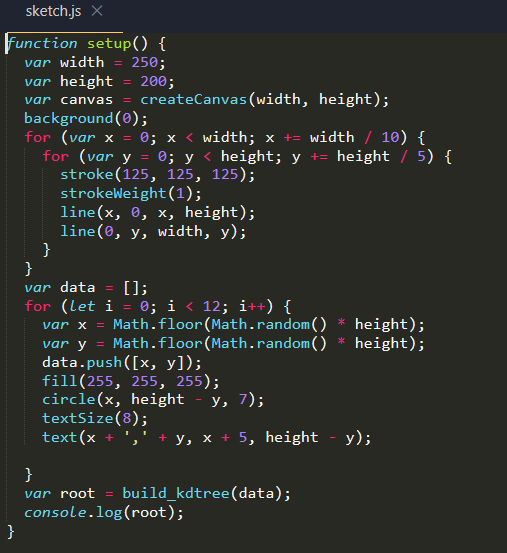
\includegraphics[width=0.5\textwidth]{images/tres.PNG}
  \caption{sketch.js}
  \label{fig:act-2}
\end{figure}

\begin{figure}[H]
  \centering
  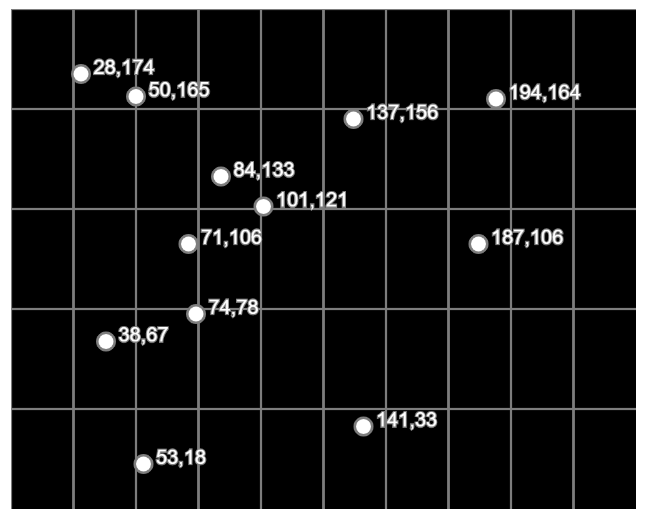
\includegraphics[width=0.6\textwidth]{images/dos.PNG}
  \caption{Puntos generados aleatoriamente}
  \label{fig:act-3}
\end{figure}

\begin{figure}[H]
  \centering
  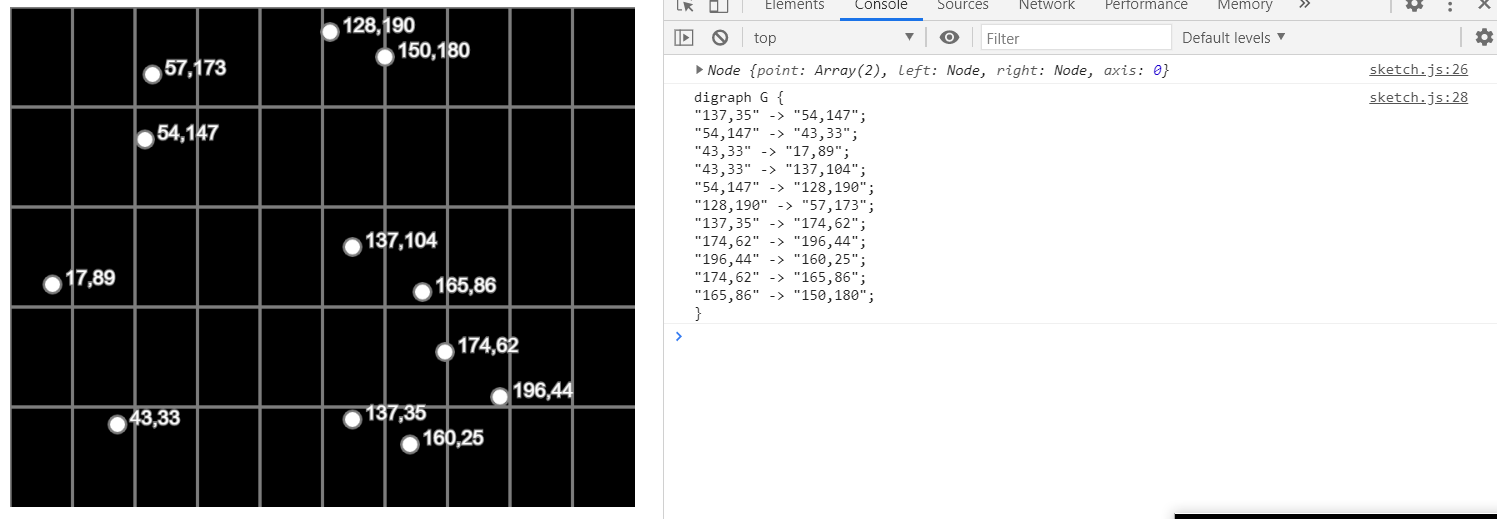
\includegraphics[width=1.1\textwidth]{images/cuatro.PNG}
  \caption{Formato dot en la consola}
  \label{fig:act-4}
\end{figure}

\subsection{Método \textit{Reconstruction}}
\doublebox{
    \begin{minipage}[c][1.2\height] [c]{1\textwidth}
    \newline
    Defina un método \textit{reconstruction}, que asignará a cada pixel su nuevo color, despues de aplicar la reducción.
    \end{minipage}
}\\
\begin{lstlisting}[language=C++,
                   directivestyle={\color{black}}
                   emph={int,char,double,float,unsigned},
                   emphstyle={\color{blue}}
                  ]
void OctreeQuantizer::reconstruction(cv::Mat &entry) {
  int canal = entry.channels();
  int filas = entry.rows;
  int columnas = entry.cols * canal;

  if (entry.isContinuous()) {
    columnas *= filas;
    filas = 1;
  }

  uchar *p;
  Node *ruta;
  int i = 0;
  while (i < filas) {
    p = entry.ptr<uchar>(i);
    int j = 0;
    while (j < columnas) {
      uchar b = p[j], g = p[j + 1], r = p[j + 2];
      ruta = root;
      for (int level = 0; level < levels; level++) {
        ruta = ruta->hijo[get_index_level(r, g, b, level)];
      }

      p[j] = (ruta->color.b) / (ruta->pixel);
      p[j + 1] = (ruta->color.g) / (ruta->pixel);
      p[j + 2] = (ruta->color.r) / (ruta->pixel);
      j += 3;
    }
    ++i;
  }
}
\end{lstlisting}
\subsection{Prueba \#1 :}
Evalue el resultado de las dos funciones implementadas anteriormente con este conjunto de datos:\\

\doublebox{
    \begin{minipage}[c][1.2\height] [c]{1\textwidth}
var data = [\newline
[40 ,70] ,\newline
[70 ,130] ,\newline
[90 ,40] ,\newline
[110 , 100] ,\newline
[140 ,110] ,\newline
[160 , 100]\newline
];\newline
var point = [140 ,90]; // query 
    \end{minipage}
}

\begin{figure}[H]
 \centering
 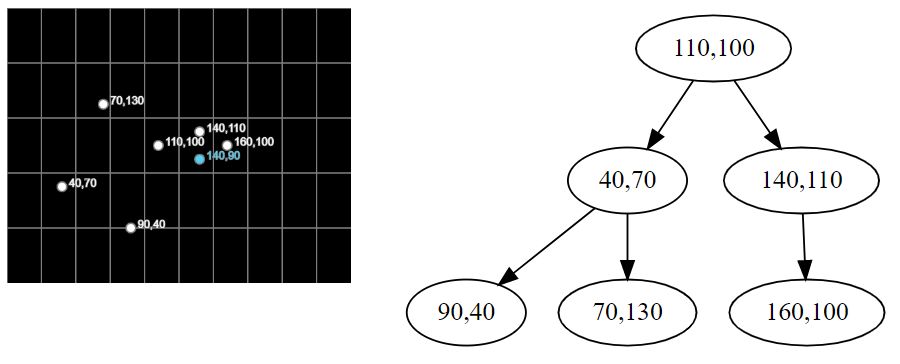
\includegraphics[width=0.9\textwidth]{images/prueba1.PNG}
 \label{fig:act-5-prueba1}
\end{figure}
\begin{itemize}
    \item closest\_point\_brute\_force
    \begin{figure}[H]
     \centering
     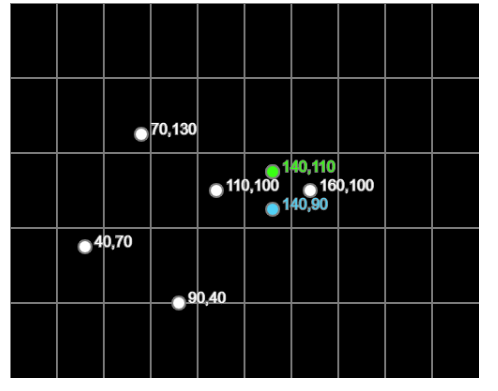
\includegraphics[width=0.6\textwidth]{images/prueba1_brute_force.PNG}
     \label{fig:act-5-1}
     \caption{Podemos apreciar el punto mas cercano de color \textcolor{green}{verde} el cual es [140,110].}
    \end{figure}
    \item naive\_closest\_point
    \begin{figure}[H]
     \centering
     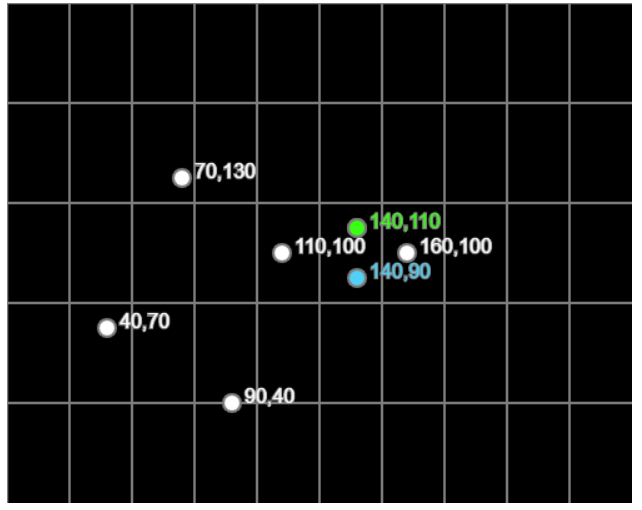
\includegraphics[width=0.6\textwidth]{images/prueba1_naive.PNG}
     \label{fig:act-5-2}
     \caption{Podemos apreciar el punto mas cercano de color \textcolor{green}{verde} el cual es [140,110].}
    \end{figure}
\end{itemize}
Observamos que en las dos funciones implementadas el punto mas cercano es [140,110]

\subsection{Resultados}
\doublebox{
    \begin{minipage}[c][1.2\height] [c]{1\textwidth}
    \newline
    Integre todo y muestre los resultados.
    \end{minipage}
}\\
\subsubsection{Imagen original}
\begin{figure}[H]
  \centering
  \includegraphics[width=0.5\textwidth]{images/original}
  \caption{Imagen original.}
  \label{fig:act-4}
\end{figure}
\subsubsection{Quantization de colores}
\begin{figure}[H]
  \centering
  \includegraphics[width=0.5\textwidth]{images/reduct}
  \caption{Reducción de colores}
  \label{fig:act-4}
\end{figure}
\subsubsection{Paleta de colores}
\begin{figure}[H]
  \centering
  \includegraphics[width=0.5\textwidth]{images/paleta}
  \caption{Paleta de colores.}
  \label{fig:act-4}
\end{figure}

%\begin{figure}[H]
%  \centering
%  \includegraphics[width=1\textwidth]{images/result}
%  \caption{Paleta de colores, imagen original y resultado despues de reducciónl.}
%  \label{fig:act-4}
%\end{figure}

\newpage
\begin{thebibliography}{8}

\bibitem{concept}
OpenCv Introduction \textit{What is OpenCv?}. \url{https://docs.opencv.org/master/d1/dfb/intro.html}.

\bibitem{concept2}
Applications: Octree Color Quantization. \url{https://en.wikipedia.org/wiki/Color_quantization}.

\end{thebibliography}

%\printbibliography[heading=bibintoc]

\end{document}